\documentclass{beamer}
%\documentclass[draft]{beamer}
%\documentclass[handout]{beamer}
%\documentclass[draft,handout]{beamer}

\usepackage[brazil]{babel}
\usepackage[latin1]{inputenc}
\usepackage[T1]{fontenc}
\usepackage{type1ec}
\usepackage{graphicx}
\usepackage{multirow}
\usepackage{ifpdf}

\ifpdf
	\usepackage{epstopdf}
\fi

%\let\newfloat=\undefined
\usepackage[portugues,boxed]{algorithm2e}
\usepackage{algorithmic}

%\newcommand{\theHalgorithm}{\arabic{algorithm}}

% Mudando o label dos algoritmos para portug�s
%\floatname{algorithm}{Algoritmo}

% Vari�veis matem�ticas
\newcommand{\C}{\mathcal{C}}
\newcommand{\Cl}{\mathcal{C}^{'}}
\newcommand{\D}{\mathcal{D}}
\newcommand{\Dl}{\mathcal{D}^{'}}
\newcommand{\Dlc}{\mathcal{D}^{'}_c}
\newcommand{\F}{\mathcal{F}}
\newcommand{\Fl}{\mathcal{F}^{'}}
\newcommand{\Flc}{\mathcal{F}^{'}_c}
\newcommand{\Fli}{\mathcal{F}^{'}_i}
\newcommand{\Flt}{\mathcal{F}^{'}_t}
\newcommand{\G}{\mathcal{G}}
\newcommand{\I}{\mathcal{I}}
\newcommand{\Il}{\mathcal{I}^{'}}
\newcommand{\M}{\mathcal{M}}
\newcommand{\Or}{\mathcal{O}}
\newcommand{\R}{\mathcal{R}}
%\newcommand{\Se}{\mathcal{S}}

\usetheme[compress]{Berlin}
%\usetheme{Berlin}

\title[Minera��o de Padr�es Freq�entes e Ortogonais]{Minera��o de Padr�es Freq�entes Ortogonais e sua Aplica��o em Classifica��o Associativa}
\author[Leandro S. Costa]{Leandro Souza Costa \\ Orientador: Wagner Meira Jr.}
\institute[DCC-UFMG]{Departamento de Ci�ncia da Computa��o \\ Universidade Federal de Minas Gerais}
\logo{\includegraphics[height=.8cm]{../thesis/img/speed}}
\date[Disserta��o de Mestrado]{Defesa de Disserta��o de Mestrado \\ \today}

\begin{document}

\setbeamercovered{transparent}

\begin{frame}
\titlepage
\end{frame}

%\section*{Sum�rio}
%\begin{frame}[shrink=5]
%\tableofcontents
%\end{frame}

\chapter{Introdu��o}

H� muito j� n�o � mais novidade o fato de que vivemos, hoje, na chamada \textbf{Era da Informa��o} (termo cunhado por Daniel Bell, pelo professor em�rito da Universidade de Harvard), que se define pelo r�pido desenvolvimento da tecnologia de informa��o, caracter�stica marcante da \textbf{Sociedade P�s-Industrial}, onde nota-se que mais importante que possuir a informa��o, � saber onde e como encontr�-la.
\par
Ao longo dos anos, o desenvolvimento tecnol�gico fez com que o constante armazenamento de dados se tornasse uma atividade f�cil e barata. A conseq��ncia deste fato � a alimenta��o de enormes bases de dados, o que proporcionou a  necessidade de se pensar em novas solu��es de ger�ncia, manuten��o e, posteriormente, acesso.
\par
Os Sistemas de Gerenciamento de Banco de Dados (\textbf{SGBD}) surgiram como uma solu��o para ger�ncia e manuten��o de bases, com o objetivo de retirar da aplica��o cliente a responsabilidade de gerenciar o acesso, a manipula��o e a organiza��o dos dados. Entretanto, embora os complexos SGBD's tenham se consolidado como eficientes sistemas na ger�ncia de complexos volumes de dados, e tratado com efici�ncia e efic�cia a recupera��o de informa��es em grandes cole��es, da exist�ncia de tais bases surgiu a necessidade de m�todos mais avan�ados de recupera��o de informa��o, como redu��o de volume de dados, extra��o da ess�ncia da informa��o armazenada, descoberta de padr�es em dados brutos, dentre outros.
\par
Como resposta � necessidade dos novos m�todos de recupera��o de informa��o, surgiu o que chamamos hoje de \textbf{Minera��o de Dados}.

\section{Minera��o de Dados}

Minera��o de dados � o resultado de um longo processo de pesquisa e desenvolvimento, considerado uma das mais importantes fronteiras entre bases de dados e sistemas de informa��o e um dos mais promissores desenvolvimentos interdisciplinares na tecnologia da informa��o \citep{Han00}. Podemos defini-la como o conjunto de m�todos n�o triviais de an�lise de dados e extra��o de informa��o potencialmente �til, impl�cita, previamente desconhecida, e suas novas formas de representa��o e visualiza��o \citep{Kumar06, Hand01, PiatetskyF91}.

Falar das solu��es encontradas na minera��o de dados para resolver os problemas citados, (agrupamento, regras associativas, etc). "Minera��o de dados � uma tecnologia usada para revelar informa��o estrat�gica escondida em grandes massas de dados". \\
fonte: http://br.geocities.com/dugimenes/mineracao.htm \\
fonte: http://pt.wikipedia.org/wiki/Minera\%C3\%A7\%C3\%A3o\_de\_dados \\
Citar \cite{Kumar06}. \\
Procurar livros, como \cite{Han00}. \\
http://books.google.com/books?hl=en\&lr=\&id=AfL0t-YzOrEC\&oi=fnd\&pg=PR21\&dq=data+mining\&ots=UuSVuVarG6\&sig=swJzbDeqSGlffWudUjXszg5vNPA\#PPP1,M1

\subsection{Padr�es Freq�entes}

�timo Survey sobre minera��o de padr�es freq�entes (possui descri��o do problema, minera��o de itemsets, espa�o de busca, regras de associa��o, algoritmo apriori fp-growth, etc...): \cite{goethals03survey}.

\subsection{Regras de Associa��o}

Artigo que fala de classifica��o e Regras de Associa��o: \cite{liu98integrating} (CBA)
O Survey tamb�m fala de regras de associa��o: \cite{goethals03survey}.
Artigo do Zaki, que fala tamb�m (CHARM): \cite{zaki99charm}.
Novos algoritmos para descoberta r�pida de regras de associa��o: \cite{DBLP:conf/kdd/ZakiPOL97}.

\section{Ortogonalidade}

Boa fonte para ortogonalidade (termo geral) - wikepedia: http://en.wikipedia.org/wiki/Orthogonal \\
Citar poucos artigos que tratam de ortogonalidade, como ORIGAMI \citep{zaki07origami}, Redundancy-Aware Top-k Patterns \citep{DBLP:conf/kdd/XinCYH06} e Orthogonal Decision Trees \citep{dutta2004orthogonal}. \\
Procurar mais fontes.

\section{Organiza��o do Documento}

�ltimo texto a ser escrito...

\chapter{Algoritmos de Classifica��o}

O artigo \cite{DBLP:conf/icde/ChengYHH07} possui uma se��o dizendo por qu� padr�es frequentes s�o bons para classifica��o.

\section{Fundamentos Te�ricos e Defini��es}

Procurar livros de minera��o de dados e artigos antigos. \\
Falar sobre regras de associa��o. \\
Falar de �rvores de decis�o.

\section{Estrat�gias eager e lazy}

Em \cite{Veloso06Lazy} O Adriano discute bem as duas estrat�gias, procurar mais artigos relacionados. \\
Descrever as duas estrat�gias, e apresentar as vantagens do lazy.

\section{M�tricas de Regras de Associa��o}

Falar sobre similaridade, cobertura, lift, leverage, etc. \\
fonte: http://www.daylight.com/meetings/emug01/Bradshaw/Similarity/YAMS.html \\
fonte: http://wwwai.wu-wien.ac.at/\%7Ehahsler/research/association\_rules/measures.html

\section{Trabalhos Relacionados}

Falar de \cite{DBLP:conf/kdd/KnobbeH06}, que obt�m, de um conjunto de itens, um itemset que particione uma base de dados o mais uniformemente poss�vel.
Falar de \cite{DBLP:conf/icde/LentSW97} ??? artigo que realiza agrupamento de regras de associa��o num espa�o bi-dimensional.
Falar de \cite{DBLP:conf/kdd/XinCYH06}, que extrai top-k padr�es minimizando a redund�ncia de um conjunto de padr�es frequentes.
Falar sobre o ORIGAMI \cite{zaki07origami}.
Falar sobre o lazy \cite{Veloso06Lazy}

\chapter{Padr�es Freq�entes e Ortogonais}
\label{chapter:ortogonalidade}

Como j� foi mencionado na se��o \ref{sec:introducao_padroes}, padr�es freq�entes s�o largamente utilizados em diversas aplica��es na �rea de minera��o de dados, incluindo regras de associa��o, classifica��o, agrupamento, indexa��o, dentre outras. Encontra-se, na literatura, uma grande quantidade de algoritmos de minera��o de padr�es freq�entes que, para muitas aplica��es, produzem resultados satisfat�rios (como os apresentados na se��o \ref{sec:introducao_trabalhos}). Entretanto, grande parte destas solu��es ainda possuem problemas n�o resolvidos.
\par
Uma das raz�es que contribuem para este fato � que, de acordo com a defini��o, qualquer sub-conjunto de um padr�o freq�ente tamb�m � freq�ente, o que faz com que o tamanho do conjunto-solu��o do algoritmo cres�a de maneira explosiva. A introdu��o de conceitos como padr�es fechados ou padr�es maximais ajudou a resolver esta quest�o, por�m, as abordagens existentes minimizam o conjunto-solu��o apenas sob a perspectiva do suporte, n�o considerando a sem�ntica dos dados, o que pode fazer com que padr�es interessantes ao usu�rio sejam retirados da solu��o durante o processo de minimiza��o do resultado.
\par
Outro desafio que ainda persiste na minera��o de padr�es freq�entes � a elimina��o de redund�ncia nos resultados obtidos. Em muitas aplica��es encontramos a necessidade de extrair um pequeno conjunto de padr�es freq�entes que tenham, n�o s� alta signific�ncia, mas tamb�m baixa redund�ncia. A signific�ncia �, em geral, definida pelo contexto da aplica��o. De acordo com \cite{DBLP:conf/kdd/XinCYH06}, alguns estudos recentes t�m se concentrado em como extrair top-$k$ padr�es com alta signific�ncia, e outros em como remover redund�ncia entre padr�es, mas poucos t�m se dedicado a obter sub-conjuntos de alta signific�ncia e baixa redund�ncia ao mesmo tempo.
\par
O objetivo da aplica��o de ortogonalidade no problema da minera��o de padr�es freq�entes � desenvolver uma t�cnica capaz de extrair um sub-conjunto de padr�es com tanto alta signific�ncia quanto baixa redund�ncia entre seus elementos.
\par
%Como j� foi mencionado no cap�tulo \ref{chapter:classificacao}, encontra-se, na literatura, diversos trabalhos relacionados com classifica��o, explorando o problema das mais variadas maneiras, e apresentando modelos diferentes, capazes de se adaptar aos diversos tipos de aplica��es existentes.
%\par
%Paralelamente, a ortogonalidade tem aparecido, em alguns dos �ltimos trabalhos de minera��o de dados, como uma forma de se resolver problemas de redund�ncia em conjuntos de padr�es freq�entes extra�dos de determinada base de dados.
%\par
%A utiliza��o de ortogonalidade para se diminuir a redund�ncia dos conjuntos de padr�es utilizados na gera��o de regras associativas aparece como uma poss�vel forma de se melhorar a efic�cia de tais classificadores. Assim, surge a motiva��o para a aplica��o de m�tricas de ortogonalidade entre padr�es no modelo de classifica��o associativa.
%\par
%Este cap�tulo apresenta as informa��es relacionadas � nova abordagem de classifica��o associativa proposta. Na se��o \ref{sec:ortogonalidade_metricas} ser�o apresentadas as m�tricas de ortogonalidade exploradas, na se��o \ref{sec:ortogonalidade_estrategias} ser�o discutidas as estrat�gias de aplica��o das m�tricas. A se��o \ref{sec:ortogonalidade_classificacao} possui uma discuss�o sobre as formas como a ortogonalidade foi utilizada dentro do modelo de classifica��o, e a se��o \ref{sec:ortogonalidade_origami} apresenta a estrat�gia ORIGAMI e adapta��o desenvolvida para o problema de classifica��o.
 
\section{M�tricas de Ortogonalidade}
\label{sec:ortogonalidade_metricas}

Para se extrair um sub-conjunto de padr�es de alta signific�ncia e baixa redund�ncia em rela��o ao conjunto original de padr�es freq�entes, � necess�rio definir m�tricas que possibilitem a avalia��o dos v�rios conjuntos-solu��o poss�veis. Na literatura, encontramos alguns exemplos de tais m�tricas. Em \cite{DBLP:conf/kdd/XinCYH06} os autores utilizam, em seus experimentos, o complemento do coeficiente de \textbf{Jaccard} \citep{jain88} aplicado � cobertura da base de dados para se obter uma medida de dist�ncia entre dois padr�es: \[D(p_1,p_2) = 1 - \frac{|TS(p_1) \cap TS(p_2)|}{|TS(p_1) \cup TS(p_2)|},\] onde $TS(p)$ � o conjunto de transa��es cobertas pelo padr�o $p$.
\par
Em \cite{zaki07origami} os autores discutem diferentes m�tricas de similaridade entre grafos, incluindo, al�m do coeficiente de \textbf{Jaccard}: \[sim(G_a, G_b) = \frac{|t(G_a) \cap t(G_b)|}{|t(G_a) \cup t(G_b)|},\] uma m�trica de dist�ncia para grafos baseada no m�ximo sub-grafo comum \citep{bunke98}: \[sim_{mc}(G_1, G_2) = \frac{|G_{mc}|}{max(|G_1|,|G_2|)},\] onde $G_{mc}$ � o maior sub-grafo comum entre $G_1$ e $G_2$.
\par
A principal caracter�sticas destas m�tricas � que elas foram desenvolvidas para avalia��o de pares de padr�es, e n�o aplic�veis em conjuntos de tamanho maior que $2$. No nosso caso, estamos interessados em m�tricas que definem a ortogonalidade de conjuntos de qualquer tamanho. Nas pr�ximas sub-se��es apresentaremos tr�s m�tricas de ortogonalidade propostas e indicadas para o problema da classifica��o associativa.

%A aplica��o da ortogonalidade no modelo de classifica��o associativa tem como principal objetivo a diminui��o de redund�ncia no conjunto de regras geradas durante a fase de treinamento. Para tanto, podem ser  naO objetivo da ortogonalidade � diminuir o n�mero de padr�es utilizados para gerar as regras de associa��o. Logo, a sua utiliza��o ....

\subsection{Estrutura dos Padr�es}
\label{sec:ortogonalidade_metricas_estrutura}

Considerando a estrutura dos padr�es, ou seja, a seq��ncia de itens pelos quais s�o definidos, dizemos que dois padr�es s�o ortogonais se eles n�o possuem itens em comum, ou seja, pode-se dizer que os padr�es $ABC$ e $DEF$ s�o ortogonais, mas $ABC$ e $CDE$ n�o o s�o, j� que o item $C$ est� presente nos dois padr�es. O mesmo pode ser aplicado a conjuntos maiores, por exemplo, os padr�es $AB$, $CD$ e $EF$ s�o ortogonais, mas os padr�es $AB$, $BC$ e $CD$ n�o o s�o.
\par
Entretanto, a simples informa��o de que um determinado conjunto de padr�es � ortogonal ou n�o � insuficiente para que um poss�vel conjunto-solu��o seja avaliado. Para tanto, � preciso desenvolver uma m�trica dada por uma fun��o $\F \rightarrow \left[0, 1\right]$ que forne�a a medida de ortogonalidade do conjunto.
\par
Uma forma de se obter esta medida, � analisar os itens dos padr�es. Sabemos que dois padr�es s�o ortogonais se eles n�o compartilham itens, ou seja, a presen�a de um mesmo item em mais de um padr�o do conjunto, intuitivamente, deve contribuir de maneira negativa para a medida de ortogonalidade do mesmo. A m�trica de ortogonalidade baseada na estrutura dos padr�es associa pesos aos itens, de modo que quanto maior a sua popularidade, menor ser� o seu peso. O resultado � dado pela m�dia dos pesos de todos os itens que fazem parte dos padr�es do conjunto.
\par
Seja $\I$ um conjunto de itens, $\D$ uma base de dados de transa��es em $\I$, $\F$ o conjunto de padr�es freq�entes em $\D$, e $\Fl$ um sub-conjunto de $\F$ ($\Fl \subseteq \F$). Chamamos de $\Il \subseteq \I$ o sub-conjunto itens que aparecem em, pelo menos, um dos padr�es de $\Fl$. Para cada item $i \subseteq \Il$ � dado um peso: \[w_i = \frac{|\Fl|-|\Fli|}{|\Fl|-1},\] onde $\Fli \subseteq \Fl$ � o sub-conjunto de padr�es de $\Fl$ que cont�m o item $i$.
\par
De acordo com esta express�o, se o conjunto possui quatro padr�es, e um item $i$ est� presente em apenas um deles, o valor do seu peso $w_i$ � equivalente a $1$. Se o item estiver presente em $3$ padr�es do conjunto, o peso $w_i$ ser� $\frac{1}{3}$. Itens compartilhados por todos os padr�es t�m peso igual a $0$.
\par
Finalmente, a ortogonalidade baseada na estrutura dos padr�es do conjunto � dada por: \[O_e = \frac{\sum_{i \subseteq \Il} w_i}{|\Il|}.\]
\par
Como exemplo, suponha um conjunto de itens $\I = \left\{A, B, C, D, E \right\}$ e um conjunto de padr�es: $\F = \left\{ AB, ABC \right\}$. Na tabela \ref{tab:item_w1} encontramos valor do peso de cada item, de acordo com a express�o apresentada. Os itens $D$ e $E$ n�o possuem pesos, pelo fato de n�o serem encontrados nos padr�es.

\begin{table}[htbp]
	\centering
		\begin{tabular}{|c|c|}
		\hline
		Itens	& Pesos	\\
		\hline
		$A$	& $0$	\\
		\hline
		$B$	& $0$	\\
		\hline
		$C$	& $1$	\\
		\hline
		$D$	& $-$	\\
		\hline
		$E$	& $-$	\\
		\hline
		\end{tabular}		
	\caption{Pesos dos Itens para Ortogonalidade Baseada na Estrutura dos Padr�es (1)}
	\label{tab:item_w1}
\end{table}

Como podemos ver, o item $C$ � o �nico que faz parte de apenas um padr�o, portanto, � associado o peso $1$ para este item. Os outros dois itens ($A$ e $B$) s�o encontrados nos dois padr�es, e por isso, possuem peso $0$. De acordo com a express�o de ortogonalidade, m�dia destes valores nos d� a medida de ortogonalidade do conjunto: $O_e = 0,33$. Agora, suponha que seja inserido o novo padr�o $BCD$ ao conjunto ($\F = \left\{ AB, ABC, BCD \right\}$). A tabela \ref{tab:item_w2} possui os novos pesos para cada item.

\begin{table}[htbp]
	\centering
		\begin{tabular}{|c|c|}
		\hline
		Itens	& Pesos	\\
		\hline
		$A$	& $0,5$	\\
		\hline
		$B$	& $0$	\\
		\hline
		$C$	& $0,5$	\\
		\hline
		$D$	& $1$	\\
		\hline
		$E$	& $-$	\\
		\hline
		\end{tabular}		
	\caption{Pesos dos Itens para Ortogonalidade Baseada na Estrutura dos Padr�es (2)}
	\label{tab:item_w2}
\end{table}

Note que o novo padr�o possui um novo item ($D$) que antes n�o era encontrado no conjunto. A inser��o de $BCD$ fez com que o peso de $A$ aumentasse, visto que este item n�o faz parte do padr�o. J� o peso de $B$ continuou o mesmo, e o novo item $D$ entrou no conjunto com peso $1$. Assim, a ortogonalidade do novo conjunto � $O_e = 0,5$.

%Dois padr�es s�o similares se possuem itens em comum, logo, dois padr�es s�o ortogonais se n�o possuem itens em comum. Mostrar exemplo: AB e CD s�o mais ortogonais que AB e BC. Fazer figura do exemplo.

\subsection{Cobertura de Transa��es}
\label{sec:ortogonalidade_metricas_transacoes}

Considerando o espa�o de transa��es, dizemos que dois padr�es s�o ortogonais se eles cobrem �reas diferentes da base de dados, ou seja, se n�o existem sobreposi��es nas coberturas de cada padr�o do conjunto.
\par
Na figura \ref{fig:covex1} temos uma representa��o de uma base de dados, e os conjuntos de transa��es cobertas por tr�s padr�es ($X$, $Y$ e  $Z$). As transa��es que fazem parte das �reas $T_X$, $T_Y$ e $T_Z$ s�o cobertas por apenas um dos padr�es ($X$, $Y$ e $Z$ respectivamente). As transa��es de $T_{XY}$ s�o cobertas por $X$ e $Y$, e as transa��es de $T_{XYZ}$ s�o cobertas pelos tr�s padr�es do exemplo. Se precisamos de padr�es que cobrem diferentes �reas da base de dados, ent�o n�s estamos interessados em maximizar $T_X$, $T_Y$ e $T_Z$, no caso do exemplo.

\begin{figure}
\centering
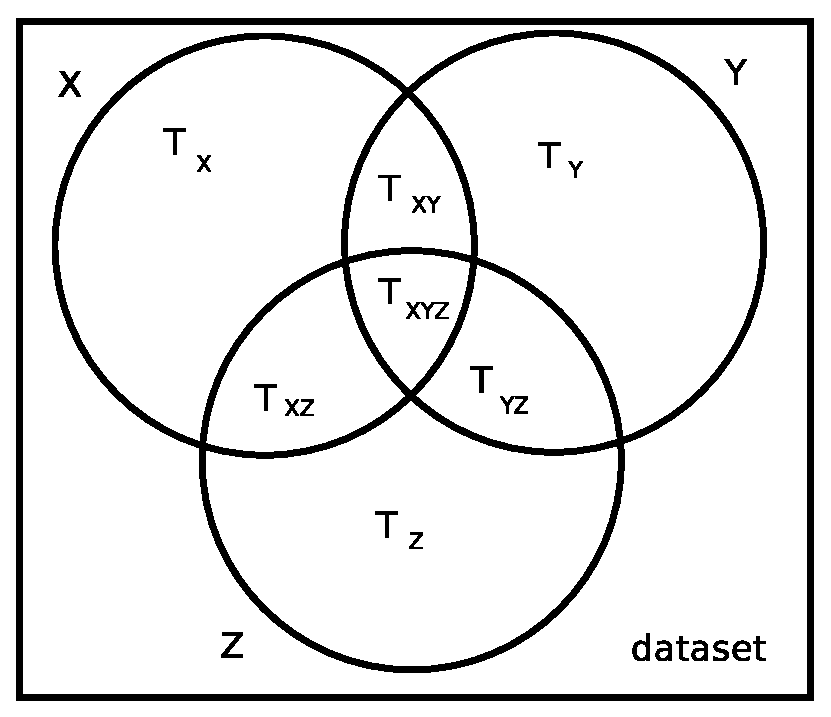
\includegraphics[width=0.5\textwidth]{img/coverage}
\caption{Visualiza��o de Cobertura de Transa��es na Base de Dados}
\label{fig:covex1}
\end{figure}

%\begin{figure}
%\centering
%\begin{picture}(180,180)
%\linethickness{0.075mm}
%\thicklines
%external frame
%\multiput(0, 0)(180, 0){2}{\line(0, 1){180}}
%\multiput(0, 0)(0, 180){2}{\line(1, 0){180}}

%circle X
%\put(90,90){\circle{170}}
%\framebox[100, 100]{teste}
%\put(-50,50){\frame{\circle{100}}
%\end{picture}
%\caption{Visualiza��o de Cobertura de Transa��es na Base de Dados}
%\end{figure}

A m�trica de ortogonalidade baseada em cobertura de transa��es pode ser calculada de maneira an�loga � relacionada com a estrutura, sendo que, neste caso, os elementos que possuem pesos a serem calculados s�o as transa��es cobertas pelos padr�es, e n�o os seus itens.
\par
Seja $\I$ um conjunto de itens, $\D$ uma base de dados de transa��es em $\I$, $\F$ o conjunto de padr�es freq�entes em $\D$, e $\Fl$ um sub-conjunto de $\F$ ($\Fl \subseteq \F$). Chamamos de $\Dl \subseteq \D$ o sub-conjunto transa��es cobertas por, pelo menos, um dos padr�es de $\Fl$. Para cada transa��o $t \subseteq \Dl$ � dado um peso: \[w_t = \frac{|\Fl| - |\Flt|}{|\Fl| - 1},\] onde $\Flt$ � o sub-conjunto de padr�es de $\Fl$ que cobrem a transa��o $t$.
\par
De acordo com esta express�o, se n�s tivermos $4$ padr�es, e uma transa��o $t$ coberta por apenas um deles, ent�o o seu peso $w_t$ ser� $1$. Se esta transa��o for coberta por dois padr�es do conjunto, o valor de $w_t$ ser� $\frac{1}{2}$. As transa��es cobertas por todos os padr�es do conjunto ter�o peso igual a $0$.
\par
A ortogonalidade baseada em cobertura de transa��es do conjunto � dada por: \[O_t = \frac{\sum_{t \subseteq \Dl} w_t}{|\Dl|}.\]
\par
Suponha uma base de dados $\D = \left\{ A, ABCD, BCDE, CDEF \right\}$, e um conjunto de padr�es $\F = \left\{ AB, BC, CD \right\}$. Na tabela \ref{tab:transacao_w1} encontramos valor do peso de cada transa��o, de acordo com a express�o apresentada. A transa��o $A$ n�o possui peso, pelo fato de n�o ser coberta por nenhum dos padr�es.

\begin{table}[htbp]
	\centering
		\begin{tabular}{|c|c|}
		\hline
		Transa��es	& Pesos	\\
		\hline
		$A$		& $-$	\\
		\hline
		$ABCD$		& $0$	\\
		\hline
		$BCDE$		& $0,5$	\\
		\hline
		$CDEF$		& $1$	\\
		\hline
		\end{tabular}		
	\caption{Pesos das Transa��es para Ortogonalidade Baseada na Cobertura de Transa��es}
	\label{tab:transacao_w1}
\end{table}

A transa��o $CDEF$ � a �nica coberta por apenas um padr�o do conjunto, portanto, � associado o peso $1$ para ela. A transa��o $BCDE$ � coberta por dois padr�es, portanto, recebe o peso $0,5$, e a transa��o $ABCD$ recebe o peso $0$, j� que ela � coberta por todos os padr�es do conjunto. A m�dia dos pesos das transa��es nos d� o valor da ortogonalidade do conjunto: $O_t = 0,5$.

\subsection{Cobertura de Classes}
\label{sec:ortogonalidade_metricas_classes}

As duas m�tricas de ortogonalidade apresentadas nas se��es \ref{sec:ortogonalidade_metricas_estrutura} e \ref{sec:ortogonalidade_metricas_transacoes} est�o relacionadas apenas com os padr�es e as transa��es da base, e podem ser utilizadas em qualquer tipo de aplica��o. J� a m�trica apresentada nesta se��o � voltada diretamente para o problema da classifica��o, pois est� relacionada �s classes das transa��es cobertas pelos padr�es do conjunto.
\par
A motiva��o para esta m�trica est� calcada na seguinte considera��o: Dois padr�es s�o ortogonais se s�o encontrados em transa��es de classes distintas na base de dados, ou seja, os conjuntos de transa��es cobertas por cada um dos padr�es n�o devem possuir classes em comum.
\par
A m�trica de cobertura de classes pode ser calculada de maneira an�loga �s relacionadas m�tricas de similaridade entre padr�es e cobertura de transa��es, sendo que, neste caso, os elementos que possuem pesos a serem calculados s�o as classes existentes nas transa��es cobertas pelos padr�es.
\par
Seja $\I$ um conjunto de itens, $\D$ uma base de dados de transa��es em $\I$, $\F$ o conjunto de padr�es freq�entes em $\D$, e $\Fl$ um sub-conjunto de $\F$ ($\Fl \subseteq \F$). Chamamos de $\Dl \subseteq \D$ o sub-conjunto transa��es cobertas por, pelo menos, um dos padr�es de $\Fl$. Seja $\C$ um conjunto de classes associadas �s transa��es de $\D$. Chamamos de $\Cl \subseteq \C$ o sub-conjunto de classes associadas �s transa��es de $\Dl$. Para cada classe $c \subseteq \Cl$ � dado um peso: \[w_c = \frac{|\Fl| - |\Flc|}{|\Fl| - 1},\] onde $\Flc$ � o sub-conjunto de padr�es de $\Fl$ que cobrem uma quantidade de transa��es de classe $c \subseteq \Cl$ maior que $90\%$ da m�dia esperada \footnote{Dado um conjunto de transa��es $\Dlc$ onde todas as transa��es possuem a classe $c$ e um conjunto de padr�es $\Fl$ em $\Dlc$, a cobertura esperada de cada padr�o para a classe $c$ � $\frac{|\Dlc|}{|\Fl|}$ (considerando que todos os padr�es s�o independentes, ou seja, ortogonais).}.
\par
De acordo com esta express�o, se n�s temos 4 padr�es, e uma classe $c$ que aparece em transa��es cobertas por apenas um deles, ent�o o seu peso $w_c$ ser� $1$. Se esta classe aparece em transa��es cobertas por dois padr�es do conjunto de maneira balanceada (por exemplo, $50\%$ das  transa��es da classe aparece em um dos padr�es, e o $50\%$ restantes no outro), o valor de $w_c$ ser� $\frac{1}{2}$. As classes que aparecem por igual em transa��es cobertas por todos os padr�es do conjunto ter�o peso igual a $0$.
\par
Por fim, a ortogonalidade baseada em cobertura de classes � dada por: \[O_c = \frac{\sum_{c \subseteq \Cl} w_c}{|\Cl|}.\]
\par
Suponha uma base de dados $\D$ em que as transa��es respectivas classes s�o encontradas na tabela \ref{tab:classe_db}.

\begin{table}[htbp]
	\centering
		\begin{tabular}{|c|c|}
		\hline
		Transa��es	& Classes	\\
		\hline
		$ABCD$		& $1$		\\
		\hline
		$ACD$		& $1$		\\
		\hline
		$BCDE$		& $1$		\\
		\hline
		$BDEF$		& $2$		\\
		\hline
		$CDE$		& $2$		\\
		\hline
		$CEF$		& $2$		\\
		\hline
		\end{tabular}		
	\caption{Base de Dados de Transa��es e Classes}
	\label{tab:classe_db}
\end{table}

Suponha um conjunto de padr�es $\F = \left\{AB, CD, EF \right\}$. Os pesos de cada classe, de acordo com a express�o apresentada, s�o encontrados na tabela \ref{tab:classe_w1}.

\begin{table}[htbp]
	\centering
		\begin{tabular}{|c|c|}
		\hline
		Classes	& Pesos	\\
		\hline
		$1$	& $1$	\\
		\hline
		$2$	& $0,5$	\\
		\hline
		\end{tabular}		
	\caption{Pesos das Classes para Ortogonalidade Baseada na Cobertura de Classes}
	\label{tab:classe_w1}
\end{table}

Como pode ser visto na tabela \ref{tab:classe_db}, a classe $1$ � coberta uma vez pelo padr�o $AB$ (transa��o $ABCD$, e tr�s vezes pelo padr�o $CD$ (transa��es $ABCD$, $ACD$ e $BCD$), totalizando $4$ coberturas. Como o conjunto de padr�es possui tamanho $3$, considerando que todos os padr�es sejam independentes, espera-se que a cobertura de classes seja homog�nea, ou seja, que cada padr�o cubra $4/3$ transa��es de cada classe. De acordo com a express�o apresentada, consideramos $\Flc$ o conjunto de padr�es que cobrem uma quantidade de transa��es da classe $c$ maior que $90\%$ da m�dia esperada (neste caso, $1,2$). Do nosso conjunto de padr�es, o �nico que satisfaz esta premissa � $CD$, que ocorre em $3$ transa��es da classe $1$. Logo, o peso dessa classe � $1$.
\par
J� a classe $2$ � coberta duas vezes pelo padr�o $CD$, e duas vezes pelo padr�o $EF$, logo, tamb�m possui cobertura esperada igual a $4/3$. Entretanto, os dois padr�es possuem cobertura desta classe acima de $90\%$ da m�dia esperada, logo, o peso dessa classe � $0,5$. A m�dia dos pesos das classes nos d� o valor da ortogonalidade do conjunto: $O_c = 0,75$.

\subsection{Utiliza��o das M�tricas}
\label{sec:ortogonalidade_estrategias}

Ap�s a introdu��o das m�tricas, � necess�rio definir como elas ser�o utilizadas para se obter a medida de ortogonalidade do conjunto. Na literatura, encontramos algumas estrat�gias interessantes.
\par
Em \cite{zaki07origami} � utilizada uma medida de ortogonalidade aplic�vel a pares de padr�es. Os autores optaram por utilizar, como m�trica do conjunto, o valor da ortogonalidade entre os seus dois elementos mais similares.
\par
Em \cite{DBLP:conf/kdd/XinCYH06} os autores utilizaram m�tricas de signific�ncia aplic�veis a padr�es e m�tricas de redund�ncia aplic�veis a pares de padr�es. O valor da fun��o que compreende as duas m�tricas � obtido pela soma das signific�ncias de cada padr�o do conjunto menos a m�dia das redund�ncias existentes entre todos os pares de padr�es.
\par
Neste trabalho, duas solu��es foram implementadas. A primeira delas � baseada na medida de ortogonalidade do conjunto, onde aplicamos as m�tricas apresentadas na se��o \ref{sec:ortogonalidade_metricas} considerando todo o conjunto-solu��o. A segunda � baseada na solu��o proposta por \cite{DBLP:conf/kdd/XinCYH06} - as m�tricas s�o aplicadas somente a pares de padr�es, e a ortogonalidade do conjunto � obtida por meio da m�dia das ortogonalidades entre todos os pares poss�veis.
\par
� f�cil perceber que as m�tricas propostas nas se��es \ref{sec:ortogonalidade_metricas_estrutura} e \ref{sec:ortogonalidade_metricas_transacoes} e \ref{sec:ortogonalidade_metricas_classes} s�o equivalentes ao complemento do coeficiente de Jaccard quando aplicadas a conjuntos de dois padr�es. Tomando a m�trica baseada na estrutura dos padr�es como exemplo, temos que a ortogonalidade do conjunto � dada pela express�o: \[O_e = \frac{\sum_{i \subseteq \Il} \left( \frac{|\Fl| - |\Fli|}{|\Fl| - 1} \right)}{|\Il|}.\] Nos casos em que o conjunto de possui necessariamente dois padr�es: \[ O_e = \frac{\sum_{i \subseteq \Il} (2 - |\Fli|)}{|\Il|}.\] Analisando a express�o acima, temos que $|\Il|$ corresponde ao tamanho do conjunto de itens encontrados nos dois padr�es, ou seja, \[|\Il| = |p_1 \cup p_2|,\] onde $\Fl = \left\{p1, p2 \right\}$, e a parcela $(2 - |\Fli|)$ ter� valor $1$ para itens que est�o presentes em apenas um dos padr�es, e $0$ para itens presentes nos dois padr�es, ou seja, \[\sum_{i \subseteq \Il} (2 - |\Fli|) = |p_1 \cup p_2| - |p_1 \cap p_2|.\] Logo, a m�trica de ortogonalidade baseada na estrutura dos padr�es, quando aplicada par-a-par, � dada pela seguinte express�o: \[O_e = 1 - \frac{\sum_{p_1, p_2 \subseteq \Fl, p_1 \neq p_2} \frac{|p_1 \cap p_2|}{|p_1 \cup p_2|}}{\frac{|\Fl| \times (|\Fl|-1)}{2}}.\]
\par
A m�trica de ortogonalidade baseada em cobertura de transa��es, quando aplicada par-a-par, � dada pela seguinte express�o: \[O_t = 1 - \frac{\sum_{p_1, p_2 \subseteq \Fl, p_1 \neq p_2} \frac{|\Dl_{p1} \cap \Dl_{p2}|}{|\Dl_{p1} \cup \Dl_{p2}|}}{\frac{|\Fl| \times (|\Fl|-1)}{2}},\] onde $\Dl_p$ � o sub-conjunto de transa��es cobertas pelo padr�o $p$.
\par
A m�trica de ortogonalidade baseada em cobertura de classes, quando aplicada par-a-par, � dada pela seguinte express�o: \[O_c = 1 - \frac{\sum_{p_1, p_2 \subseteq \Fl, p_1 \neq p_2} \frac{|\Cl_{p1} \cap \Cl_{p2}|}{|\Cl_{p1} \cup \Cl_{p2}|}}{\frac{|\Fl| \times (|\Fl|-1)}{2}},\] onde $\Cl_p$ � o sub-conjunto de classes cujas transa��es s�o cobertas pelo padr�o $p$ $90\%$ acima da m�dia esperada.

%Breve introdu��o, falar sobre m�tricas utilizadas por \cite{DBLP:conf/kdd/XinCYH06} e \cite{zaki07origami}.

%\subsection{Ortogonalidade por conjunto}

%Apresentar e discutir as express�es: \\
%Similaridade: Express�o que d� um peso para cada item encontrado nos padr�es do conjunto; \\
%Cobertura de Transa��es: Express�o que d� um peso para cada transa��o coberta pelo conjunto de padr�es; \\
%Cobertura de Classes: Express�o que d� um peso para cada classe encontrada nas transa��es cobertas pelos padr�es.

%\subsection{Ortogonalidade Par-a-par}

%Discutir as express�es par a par (similaridade pode ser dada por interse��o sobre uni�o de elementos, ortogonalidade pode ser dada por 1 - similaridade): \\
%Ortogonalidade por itens: Quantidade de itens que aparecem em apenas um dos padr�es / quantidade de itens que aparecem nos dois padr�es. \\
%Ortogonalidade por cobertura de transa��es: Quantidade de transa��es cobertas por apenas um dos padr�es / quantidade de transa��es cobertas pelos dois padr�es. \\
%Ortogonalidade por cobertura de classes: Mais complicado: Ortogonalidade � a m�dia das raz�es entre a diferen�a das coberturas e a maior cobertura de cada classe. 

\section{Classifica��o Associativa e Ortogonalidade}
\label{sec:ortogonalidade_classificacao}

Como j� foi dito na se��o \ref{sec:introducao_objetivos}, a utiliza��o da ortogonalidade no problema da classifica��o associativa tem como objetivo aumentar a efetividade das classifica��es, como conseq��ncia da diminui��o da redund�ncia e da ambig�idade das regras. Uma das formas de se fazer isso seria aplicar ortogonalidade no conjunto de regras geradas pelo classificador. Dessa forma, seria poss�vel extrair, de todo o conjunto de regras obtidas, apenas um sub-conjunto representativo de regras com alta signific�ncia e baixa redund�ncia, e a partir destas, realizar a classifica��o das inst�ncias de teste.
\par
Esta proposta � apresentada em \cite{DBLP:conf/kdd/XinCYH06}, onde � discutido utiliza��o de ortogonalidade aplicada a \textit{prefetch} de blocos de acesso a disco. Os autores consideram a similaridade de duas regras igual a $0$ quando os termos conseq�entes s�o diferentes, e igual ao coeficiente de Jaccard aplicado aos termos antecedentes quando os conseq�entes s�o iguais.
\par
� poss�vel aplicar este modelo no problema da classifica��o associativa. Nesse caso, seria considerado como m�trica de ortogonalidade entre duas regras o valor m�ximo ($1$) se as classes para as quais elas apontam s�o diferentes, e o valor inversamente proporcional ao coeficiente de Jaccard (ou alguma outra m�trica qualquer) aplicado aos termos antecedentes se as classes para as quais elas apontam s�o iguais. Dessa forma, estar�amos gerando todas as regras poss�veis, a partir do conjunto de padr�es freq�entes obtidos por meio de um determinado suporte, e extraindo um sub-conjunto que consiste apenas das mais representativas, para ent�o realizar a classifica��o da inst�ncia de teste.
\par
Neste trabalho, por�m, optamos por aplicar a ortogonalidade n�o ao conjunto de regras geradas, mas sim ao conjunto de padr�es utilizados para gerar as regras. A id�ia � gerar regras a partir de um sub-conjunto dos padr�es freq�entes obtidos, que consiste apenas dos padr�es ortogonais. A principal diferen�a desta abordagem, em rela��o � anterior, � que as m�tricas de ortogonalidade s�o aplicadas apenas aos termos antecedentes - os padr�es, ou seja, as classes n�o s�o consideradas.
\par
As tr�s m�tricas descritas na se��o \ref{sec:ortogonalidade_metricas} foram utilizadas neste trabalho. A m�trica baseada na estrutura dos padr�es foi utilizada com o objetivo de se encontrar um sub-conjunto de padr�es que represente bem todo o conjunto de padr�es freq�entes. Por ser uma m�trica que considera o conjunto de itens, ela se aplica ao espa�o dos padr�es, n�o considerando a sua rela��o com as transa��es da base. Neste caso, estamos interessados em diminuir, principalmente, a redund�ncia das regras, ou seja, n�o gerar regras com um alto n�vel de similaridade entre os termos antecedentes.
\par
A cobertura de transa��es foi utilizada com o objetivo de se encontrar padr�es ortogonais no espa�o de transa��es. Com esta m�trica, espera-se obter um sub-conjunto de padr�es que cobrem a base de dados com o m�nimo de sobreposi��es poss�vel, ou seja, que as regras geradas por cada um destes padr�es apontem para transa��es distintas da base. A inten��o, neste caso, � diminuir a ambig�idade das regras, al�m da redund�ncia.
\par
A cobertura de classes � uma m�trica definida especialmente para o problema da classifica��o, j� que ela considera as classes das transa��es da base de treinamento para definir o conjunto de padr�es ortogonais. Esta m�trica � uma adapta��o da cobertura de transa��es, visto que ela tamb�m est� centrada na base de dados. A diferen�a � que, ao contr�rio da anterior, esta m�trica analisa as classes, e n�o as transa��es cobertas pelos padr�es. A motiva��o � que n�o basta extrair padr�es que cobrem transa��es distintas da base de dados se estas transa��es possuem classes coincidentes. Esta m�trica tenta garantir que as regras geradas pelo conjunto-resultado de padr�es apontem para classes distintas. A inten��o, como na m�trica anterior, � diminuir a ambig�idade das regras, al�m da redund�ncia.

%Falar sobre como utilizar o conceito de ortogonalidade em algoritmos de regras de associa��o:
%Ortogonalidade por itens: Motiva��o: Encontrar um conjunto de padr�es ortogonais que representem bem todo o conjunto de padr�es freq�entes, e que gere regras n�o redundantes;
%Ortogonalidade por cobertura de transa��es: Encontrar um conjunto de padr�es que cubram �res ortogonais, e dessa forma, distintas da base de dados, diminuindo a redund�ncia de informa��es durante a gera��o das regras, e mais que isso, diminuindo a possibilidade de encontrar regras redundantes;
%Ortogonalidade por cobertura de classes: Encontrar um conjunto de padr�es que aparecem em transa��es de classes distintas, ou seja, padr�es que apontam para classes distintas. A id�ia � gerar regras n�o redundantes, e obter a classifica��o das regras de maior peso no ranking.

\subsection{Utiliza��o de Ortogonalidade no LAC}

O \textbf{LAC} (\textit{Lazy Associative Classifier}) � uma implementa��o da abordagem \textit{lazy} proposta em \cite{Veloso06Lazy}. A abordagem de classifica��o associativa \textit{lazy} obt�m o conjunto de regras de associa��o relacionadas a cada inst�ncia de teste separadamente. Para tanto, ela cria uma proje��o da base de treinamento apenas com as transa��es que possuem itens em comum com a inst�ncia de teste. A partir desta proje��o, a abordagem obt�m um conjunto de padr�es freq�entes, de acordo com determinado suporte fornecido pelo usu�rio, e com estes padr�es, gera as regras de associa��o utilizadas durante a tarefa de classifica��o.
\par
A ortogonalidade pode ser utilizada de v�rias maneiras no \textit{lazy}, por exemplo, � poss�vel extrair, \textit{apriori}, o conjunto de itens ortogonais da base de treinamento, considerando cobertura de transa��es, ou cobertura de classes, e, para cada inst�ncia de teste, obter a proje��o da base de treinamento considerando apenas os itens que fazem parte do conjunto ortogonal. Esta seria uma boa op��o para diminuir o espa�o de busca durante a obten��o do conjunto de padr�es freq�entes nos casos em que as bases de dados s�o muito densas.
\par
Uma outra maneira seria extrair o conjunto de itens ortogonais, n�o de toda a base de treinamento, mas sim de cada inst�ncia no momento do teste. Entretanto, tanto esta forma quanto a anterior ainda possibilitaria a gera��o de conjuntos de regras redundantes, j� os itens obtidos, mesmo mantendo a caracter�stica de ortogonalidade entre si, poderiam gerar padr�es similares.
\par
Sendo assim, a forma escolhida neste trabalho foi continuar utilizando todos os itens da inst�ncia de teste para gerar a proje��o da base. A partir destes, obter o conjunto de padr�es freq�entes e ent�o, extrair o sub-conjunto de padr�es ortogonais, com os quais s�o geradas as regras de associa��o.

\subsection{Heur�stica de Obten��o de Conjuntos Ortogonais}

O problema de se encontrar o sub-conjunto de padr�es com maior m�trica de ortogonalidade, dado o conjunto de padr�es freq�entes, � n�o polinomial, visto que todas as combina��es de todos os tamanhos poss�veis devem ser testadas para se chegar ao resultado final. Portanto, foi desenvolvida uma heur�stica gulosa que inicia com um conjunto ortogonal de dois elementos, e iterativamente, tenta obter um novo conjunto com um elemento a mais, acrescentando padr�es candidatos e realizando modifica��es para que a m�trica de ortogonalidade seja maximizada.
\par
Esta abordagem � semelhante ao que foi proposto em \cite{zaki07origami}. Este artigo apresenta um algoritmo que considera o conjunto de padr�es freq�entes como um grafo em que cada v�rtice representa um padr�o, e uma aresta entre dois v�rtices representa a similaridade entre os padr�es. No entanto, s� s�o representadas as arestas que possuem similaridade menor que $\alpha$ (par�metro do algoritmo). O objetivo da heur�stica � encontrar um clique de tamanho m�ximo neste grafo. Para tanto, o algoritmo escolhe um v�rtice aleatoriamente e o adiciona no conjunto-solu��o. Ap�s este passo, o algoritmo passa a visitar os vizinhos dos v�rtices que j� fazem parte da solu��o, escolhendo sempre o melhor candidato para adicionar ao conjunto, at� que n�o haja mais v�rtices para se adicionar.
\par
No nosso caso, n�o utilizamos o par�metro $\alpha$, limite inferior para a m�trica de ortogonalidade. Sendo assim, todos os padr�es s�o candidatos ao conjunto-resultado. A obten��o do conjunto ortogonal de padr�es � realizada de forma iterativa, onde no in�cio da execu��o, o algoritmo inicializa o conjunto-solu��o com apenas um elemento, e a m�trica de ortogonalidade do conjunto com o valor $0$ (zero), e ent�o come�a o ciclo de itera��es em que, a cada etapa:

\begin{enumerate}
	\item Um novo elemento � inclu�do ao conjunto;
	\item � realizada uma busca por todo o conjunto de padr�es que n�o fazem parte do conjunto-solu��o. Durante este procedimento, cada padr�o verificado � inclu�do na solu��o, substituindo, neste conjunto, o elemento que mais se assemelha �quele. Se a m�trica de ortogonalidade do conjunto melhorou, o algoritmo mant�m a troca. Se n�o, a troca � desfeita, e o pr�ximo padr�o da seq��ncia � verificado;
	\item Ao final do processo, o algoritmo compara a m�trica de ortogonalidade obtida com a m�trica do conjunto anterior (que possu�a um elemento a menos). Se a m�trica se manteve, ou melhorou, o algoritmo mant�m o novo conjunto como solu��o, e volta ao in�cio do ciclo. Se n�o, o algoritmo termina o ciclo, e o conjunto anterior � dado como resultado.
\end{enumerate}

A ordem como o algoritmo percorre o conjunto de padr�es em cada itera��o possui uma grande influ�ncia no algoritmo, pois um novo padr�o verificado s� far� parte do conjunto solu��o se a ortogonalidade do novo conjunto for maior que a do antigo, logo, em caso de empate, os primeiros padr�es ter�o prefer�ncia sobre os �ltimos. Cinco formas diferentes de ordena��o do conjunto de padr�es freq�entes foram implementadas:

\begin{enumerate}
	\item Ordena��o lexicogr�fica crescente;
	\item Ordena��o lexicogr�fica decrescente;
	\item Ordena��o por tamanho crescente;
	\item Ordena��o por tamanho decrescente;
	\item Nenhuma ordena��o.
\end{enumerate}

As ordena��es lexicogr�ficas foram utilizadas para se diminuir a dist�ncia entre dois padr�es da seq��ncia, fazendo com que a modifica��o do conjunto-solu��o seja realizada de forma suave. Espera-se que, neste caso, a diferen�a estrutural entre dois padr�es consecutivos do conjunto durante cada itera��o seja a menor poss�vel. As ordena��es por tamanho foram utilizas para dar prioridade, hora aos maiores padr�es (ordena��o decrescente), hora aos menores padr�es (ordena��o crescente).

O pseudo-c�digo do algoritmo de classifica��o associativa baseada em ortogonalidade \textbf{OLAC} (\textit{Orthogonal Lazy Assiciative Classifier}) pode ser visto no algoritmo \ref{alg:olac}.\

\begin{algorithm}
\caption{OLAC}
\label{alg:olac}
\begin{algorithmic}[1]

\REQUIRE $\D, \sigma$
\STATE $\F \leftarrow FindFrequentPatterns (\D, \sigma)$
\STATE $Sort (\F)$
\STATE $\Or \leftarrow GetFirstAvailablePattern (\F)$
\REPEAT
	\STATE $rate \leftarrow GetOrthogonalityRate (\Or)$
	\STATE $\Or_{try} \leftarrow \Or \cup GetFirstAvailablePattern (\F)$
	\STATE $rate_{try} = GetOrthogonalityRate (\Or_{try})$
	\FOR {$P \in \F, P \notin \Or_{try}$}
		\STATE $S \leftarrow GetMoreSimilar (\Or, P)$
		\STATE $\Or_{try} \leftarrow \Or_{try} \cup P \ \backslash \ S$
		\STATE $rate_{tmp} = GetRate (\Or)$
		\IF {$rate_{tmp} \leq rate_{try}$}
			\STATE $\Or_{try} \leftarrow \Or_{try} \cup S \  \backslash \  P$
		\ELSE
			\STATE $rate_{try} \leftarrow rate_{tmp}$
		\ENDIF
	\ENDFOR
	\IF {$rate_{try} \geq rate$}
		\STATE $\Or \leftarrow \Or_{try}$
	\ENDIF
\UNTIL {$rate_{try} < rate$}
\STATE $\R \leftarrow \Or$

\end{algorithmic}
\end{algorithm}

\section{Estrat�gia ORIGAMI}
\label{sec:ortogonalidade_origami}

O \textbf{ORIGAMI} � um algoritmo para minera��o de grafos apresentado em \cite{zaki07origami}. Neste artigo, os autores introduzem a defini��o de conjuntos $\alpha$-ortogonais e $\beta$-representativos, e apresentam o novo paradigma de minera��o de conjuntos de grafos ortogonais com foco nos padr�es, e n�o nas transa��es.

\subsection{Defini��o de alfa-ortogonalidade}
\label{sec:ortogonalidade_origami_definicao}

Seja $\F$ o conjunto de todos os sub-grafos freq�entes de uma cole��o. Seja $sim : \F \times \F \rightarrow \left[0, 1\right]$ uma fun��o bin�ria e sim�trica que retorna a \textit{similaridade} entre dois grafos, por exemplo, a similaridade entre dois grafos $G_a$ e $G_b$ baseada no m�ximo sub-grafo comum \citep{bunke98} � dada por \[sim(G_a, G_b) = \frac{|G_c|}{max(|G_a|, |G_b|)},\] onde $G_c$ � o m�ximo sub-grafo comum entre $G_a$ e $G_b$.
\par
Dada uma cole��o de grafos $\G$, e um limite superior para similaridade $\alpha \in \left[0, 1\right]$, dizemos que o sub-conjunto de grafos $\R \subseteq \G$ � \textbf{$\alpha$-ortogonal} em rela��o a $\G$ se, e somente se, para quaisquer $G_a, G_b \in \R, sim(G_a, G_b) \leq \alpha$ e para qualquer $G_a \in \R$ e qualquer $G_b \in \G \backslash \R, sim(G_a, G_b) > \alpha$.
\par
Dada uma cole��o de grafos $\G$,um conjunto $\alpha$-ortogonal $\R \subseteq \G$ e um dado limite inferior para similaridade $\beta \in \left[0, 1\right]$, dizemos que $\R$ \textbf{representa} um grafo $G \in \G$ se existe algum $G_a \in \R$ tal que $sim(G_a, G) \geq \beta$. Seja $\Upsilon(\R,\G) = \left\{G \in \G : \exists G_a \in \R, sim(G, G_a) \geq \beta\right\}$, dizemos que $\R$ � um conjunto $\beta$-representativo para $\Upsilon(\R, \G)$.
\par
Dada uma cole��o de grafos $\G$ e o seu conjunto $\alpha$-ortogonal e $\beta$-representativo $\R$, chamamos de \textbf{conjunto res�duo} de $\R$ o conjunto de padr�es n�o representados em $\G$, dado como $\Delta(\R, \G) = \G \backslash \left\{ \R \cup \Upsilon(\R, \G) \right\}$, o \textit{res�duo} de $\R$ � definido como a cardinalidade do seu conjunto res�duo $|\Delta(\R, \G)|$. Finalmente, definimos a m�dia de similaridade do res�duo de $\R$ como $ars(\R, \G) = \frac{\sum_{G_b \in \Delta(\R, \G)} {max_{G_a \in \R} \left\{sim(G_a, G_b)\right\}}}{|\Delta(\R, \G)|}$.
\par
Note que, por defini��o, $\alpha < ars(\R, \G) < \beta$, j� que para quaisquer $G_a \in \R$ e $G_b \in \Delta(\R, \G), sim(G_a, G_b) \in \left(\alpha, \beta \right)$.
\par
O objetivo dos autores � encontrar conjuntos de grafos $\alpha$-ortogonais e $\beta$-representativos em rela��o ao conjunto de sub-grafos maximais $\M$. Como o conjunto de padr�es maximais prov� uma s�ntese de todos os padr�es freq�entes, e com uma quantidade bem menor de padr�es, parece razo�vel tentar um conjunto representativo ortogonal em rela��o �quele. Entretanto, como encontrar todos os sub-grafos maximais em aplica��es reais pode se tornar um problema intrat�vel, os autores optaram por utilizar um sub-conjunto do conjunto de sub-grafos maximais $\widehat{\M} \subseteq \M$. Logo, o problema pode ser definido da seguinte forma:

\begin{problem}[Minera��o de grafos $\alpha$-ortogonais e $\beta$-representativos]
Dado um sub-conjunto $\widehat{\M}$ do conjunto de grafos maximais $\M$ de uma cole��o de grafos $\G$, um limite superior para similaridade $\alpha$ e um limite inferior para similaridade $\beta$, encontre o melhor sub-conjunto $\R$ que minimize o res�duo $|\Delta(\R, \widehat{\M})|$.
\end{problem}

\subsection{Estrat�gia de Ortogonalidade}

A utiliza��o dos par�metros adicionais $\alpha$ e $\beta$ pelo ORIGAMI enriquece o modelo de conjuntos ortogonais. O par�metro $\alpha$ permite que a medida da ortogonalidade seja controlada, fazendo com que o conjunto-solu��o se aproxime ou se distancie do conjunto de padr�es freq�entes de acordo com o valor escolhido para $\alpha$. J� o par�metro $\beta$ permite medir a representatividade do conjunto em rela��o ao restante dos elementos que n�o fazem parte da solu��o.
\par
Dependendo dos valores escolhidos para os dois par�metros, duas variantes do problema s�o identificadas:

\begin{itemize}
	\item{Caso I ($\beta \leq \alpha$):} Pela defini��o de conjunto $\alpha$-ortogonal, $G_a \in \R$ e $G_b \in \widehat{\M} \backslash \R$ implica em $sim(G_a, G_b) > \alpha \geq \beta$. Logo, temos que $\Upsilon(\R, \widehat{\M}) = \widehat{\M} \backslash \R$, de onde temos que $\Delta(\R, \widehat{\M}) = 0$. Ent�o, quando $\beta \leq \alpha$, o res�duo de qualquer conjunto $\alpha$-ortogonal $\R$ � $0$, o que implica que qualquer conjunto $\alpha$-ortogonal � �timo, considerando o res�duo;
	\item{Caso II ($\beta > \alpha$):} Este � o caso geral, onde um conjunto $\alpha$-ortogonal $\R$ pode n�o ser um conjunto $\beta$-representativo para alguns grafos em $\widehat{\M}$. Em outras palavras, quando $\beta > \alpha$, o res�duo $|\Delta(\R, \widehat{\M})| \geq 0$; logo, a solu��o �tima � o conjunto de padr�es ortogonais que minimiza o res�duo. Um caso especial de $\beta > \alpha$ ocorre quando $\beta = 1$. Neste caso, cada elemento do conjunto $\alpha$-ortogonal representa somente a si mesmo, e o res�duo � dado por $|\Delta(\R, \widehat{\M})| = |\widehat{\M} \backslash \R|$.
\end{itemize}

O algoritmo ORIGAMI realiza a minera��o de padr�es ortogonais em dois passos distintos. O primeiro passo consiste em encontrar, utilizando uma heur�stica rand�mica, um sub-conjunto dos padr�es maximais da base de dados. O segundo consiste em obter, novamente com o aux�lio de uma heur�stica rand�mica, um conjunto ortogonal e representativo que minimize o res�duo. O pseudo-c�digo do ORIGAMI pode ser visto no algoritmo \ref{alg:origami}.

\begin{algorithm}
\caption{ORIGAMI}
\label{alg:origami}
\begin{algorithmic}[1]

\REQUIRE $\D, \sigma, \alpha, \beta$
\STATE $EM \leftarrow EdgeMap (\D)$
\STATE $\F_1 \leftarrow FindFrequentEdges (\D, \sigma)$
\STATE $\widehat{\M} \leftarrow 0$
\WHILE {$\neg StopCondition ()$}
	\STATE $M \leftarrow RandomMaximalGraph (\D, \F_1, EM, \sigma)$
	\STATE $\widehat{\M} \leftarrow \widehat{\M} \cup M$
\ENDWHILE
\STATE $\R \leftarrow OrthogonalRepresentativeSets (\widehat{\M}, \alpha, \beta)$

\end{algorithmic}
\end{algorithm}

%  , permitindo que a caracter�stica do conjunto ortogonal seja controlada. O par�metr $\alpha$ permite
%Falar das vantagens de alfa e beta.
%Falar da estrat�gia ale�t�ria, das m�tricas, mostrar o algoritmo.

\subsection{Adapta��o do Algoritmo}
\label{sec:ortogonalidade_origami_adaptacao}

Foi realizada a implementa��o do algoritmo ORIGAMI adaptado ao problema de classifica��o associativa utilizando as m�tricas apresentadas na se��o \ref{sec:ortogonalidade_metricas}.
\par
Como heur�stica de obten��o do conjunto de padr�es maximais, o algoritmo inicia a execu��o com o conjunto-resultado vazio e, a cada itera��o, tenta obter o maior padr�o freq�ente poss�vel adicionando a ele, aleatoriamente, itens que fazem parte da inst�ncia de teste, at� que n�o seja mais poss�vel adicionar nenhum novo item, ou a condi��o de parada local seja atingida. Se, durante a obten��o aleat�ria dos itens, o item selecionado j� ter sido utilizado, ou n�o gerar um novo padr�o freq�ente, o algoritmo decrementa um contador de tentativas. A condi��o de parada local para a gera��o de novos padr�es maximais � que, durante este processo, o n�mero m�ximo de escolhas erradas dos itens n�o pode ser maior que o tamanho da inst�ncia de teste.
\par
Ao obter um novo padr�o maximal, o algoritmo tenta inseri-lo no conjunto-solu��o. Esta opera��o consiste em remover do conjunto todos os sub-padr�es do novo candidato, e inserir o candidato caso nenhum dos padr�es que ainda existem na solu��o seja super-padr�o dele. A condi��o de parada para o algoritmo � que, durante todo o processo, o n�mero m�ximo de padr�es candidatos n�o maximais ou j� inseridos no conjunto-solu��o n�o pode ser maior que o tamanho da inst�ncia de teste.
\par
Como heur�stica para obten��o do conjunto ortogonal, o algoritmo inicia a execu��o com o valor de res�duo igual a $0$ (zero) e, a cada itera��o, tenta obter um conjunto ortogonal adicionando a ele, aleatoriamente, padr�es maximais obtidos no primeiro passo do algoritmo, at� que n�o seja mais poss�vel acrescentar novos padr�es, ou a condi��o de parada local seja atingida. Se, durante a obten��o dos padr�es, o padr�o selecionado j� ter sido utilizado, ou n�o possuir similaridade menor que $\alpha$ para com todos os outros padr�es do conjunto-solu��o, o algoritmo decrementa um contador de tentativas. A condi��o de parada local para a gera��o de conjuntos ortogonais � que, durante este processo, o n�mero m�ximo de escolhas erradas de padr�es n�o pode ser maior que a quantidade de padr�es maximais total.
\par
Ao obter um novo conjunto ortogonal, o algoritmo calcula o valor do seu res�duo. Se este valor � menor que o atual, o res�duo � atualizado, e o conjunto-solu��o passar a ser o conjunto ortogonal rec�m-encontrado. A condi��o de parada para o algoritmo � que, durante todo o processo, o n�mero m�ximo de conjuntos ortogonais candidatos que n�o melhoram o resultado n�o pode ser maior que a quantidade de padr�es maximais total.
\include{avaliacao}
\chapter{Conclus�o}

\section{Resumo}
\section{Trabalhos Futuros}

%\section{Exemplo de Execução da Heurística de Obtenção de Conjuntos Ortogonais}

\begin{frame}
	\begin{itemize}[<+-| alert@+>]
		\item $\F = \{A, B, BC, ABC\}$
		\item $Sort (\F)$
		\item $\F = \{ABC, BC, A, B\}$
	\end{itemize}
\end{frame}

\begin{frame}
	\begin{itemize}[<+-| alert@+>]
		\item $\F = \{ABC, BC, A, B\}$
		\item $Or = \{ABC, BC\}$
	\end{itemize}
\end{frame}

\begin{frame}
	\begin{itemize}[<+-| alert@+>]
		\item $\F = \{ABC, BC, A, B\}$
		\item $Or = \{ABC, BC\}$
	\end{itemize}
\end{frame}


\end{document}
